% !TEX root = ejemplo.tex

\chapter{Un poco de memoir}


\section{Lo básico}
La clase \texttt{tesisFC} tiene como base a \textit{memoir}. La motivación es poder configurar de manera fácil los ascpectos del documento sin tener que usar paquetería adicional. Así, cuando el usuario cargue un paquete es poco probable que cause alguna incompatibilidad.

\textit{Memoir} es una clase configurable, es decir, no hace falta cargar paquetes adicionales para hacer un diseño completo de cómo se verá nuestro
documento. Además puede servir tanto para \textit{book} como para \textit{article} la opción por defecto es una salida estilo \textit{book}, para cambiar al diseño estilo \textit{article} basta poner la opción \texttt{article} como opción a la clase. A diferencia de las clases
estándar donde hacer un cambio de \textit{book} a \textit{article} seguramente causará problemas (por ejemplo \verb|\chapter{...}| no está
definido en article), en \textit{memoir} no existe ese problema. Otra ventaja inmediata es que el ambiente \texttt{abstract} estará definido para \textit{book}.

La tabla de contenidos esta formada por el comando
\verb|\tableofcontents*|. Esta versión con estrella es única de memoir y su
utilidad es que no aparezca una entrada para la tabla de contenidos en la
tabla de contenidos.

Otra ventaja de \textit{memoir} es que no hace falta redefinir
\verb|\cleardoublepage| para que las páginas pares ``vacías'' antes de un
nuevo capítulo estén en blanco. La clase ya lo hace por defecto. Además, la
clase tiene las opciones \texttt{openright} para que los capítulos empiecen
en las paginas impares, \texttt{openleft} para que empiecen en las pares y
\texttt{openany} para que empiecen en la siguiente página sin importar su
paridad.

\textit{Memoir} tiene predefinidos muchos estilos de capítulo, en este documento se está usando \texttt{madsen}. Memoir tiene
definidos muchos más estilos de salida por defecto, estos pueden verse en
\url{http://www.ebookation.com/wp-content/uploads/2010/03/memoirchapstyles.pdf}

Modifique el tamaño y la posición de la caja de texto para obtener una linea de texto suficientemente grande como evitar tantos cortes de palabra, pero no ta grande como para que sea difícil pasar de una lína a otra.

Si notan como está formado un libro, el bloque de texto no está centrado
en la página. Comúnmente el margen de la espina (donde se juntan las
páginas de un libro) es la mitad que el margen de la orilla (el opuesto a
la espina). Lo mismo sucede con los margenes superior e inferior, donde el
superior es más chico que el inferior. Tomamos en cuenta estos detalles en
la formación de este documento.

También cambié cabeceras y pies, esta vez fue mínimo pero aún así es
suficiente para ver cómo cambiar cabeceras y pies (ver archivo \texttt{.cls}).

Menciono de nuevo que \textit{memoir} es una clase configurable y tiene de
manera nativa capacidades mayores o iguales a
las de los siguientes paquetes
\begin{center}
  \autocols{c}{6}{l}{abstract, appendix, booktabs, ccaption, chngcntr, chngpage, enumerate, epigraph, framed, ifmtarg, index, makeidx, moreverb, needspace, newfile, nextpage, parskip, patchcmd, setspace, shortvrb, showidx, titleref, titling, tocbibind, tocloft, verbatim, verse}
\end{center}
También tiene las capacidades, aunque con comandos diferentes, de los siguientes paquetes
\begin{center}
  crop, fancyhdr, geometry, sidecap, subfigure, titlesec
\end{center}
Por último, la clase carga los siguientes paquetes
\begin{center}
  array, dcolumn, delarray, etex, iftex, tabularx, textcase (con la opción \texttt{overload})
\end{center}
Así que no hace falta cargar ninguno de estos, de esta manera es más fácil
tener compatibilidad de paquetes.

\textit{Memoir} puede crear índices de manera relativamente sencilla, en este ejemplo
haremos uno de términos o alfabético y uno de nombres. Para esto se escribió
en el preámbulo
\begin{flushleft}
  \verb|\makeindex|\\
  \verb|\makeindex[names]|
\end{flushleft}
luego una entrada en el índice de términos se crea con el comando
\verb|\index{término}| término\index{término}. Este índice puede crear
subtérminos de la siguiente manera subtérmino\index{término!subtérmino} y
uno más subsubtérmino\index{término!subtérmino!subsubtérmino} (ver código
fuente).

Ahora una entrada para el índice de nombres
Grothendieck\index[names]{Grothendieck}. Nota que en este índice se
específico que pertenece al índice de nombres con el parámetro opcional
\texttt{[names]}.

Al final del archivo principal se puede ver cómo se imprimieron.


\section{Un poco más}
Primero veamos cómo hacer subfiguras con memoir, es decir, sin usar el paquete
\texttt{subfigure} o \texttt{subcaption}. Primero necesitamos escribir
\begin{flushleft}
  \verb|\newsubfloat{figure}|
\end{flushleft}
en el preámbulo. Este comando activará todo lo necesario para hacer
subfiguras, por ejemplo en la figura~\ref{fig:vect} hay
una forma de hacerlas usando el comando \verb|\subcaption{...}| para poner
los subtítulos correspondientes. También es posible hacer como en el
siguiente ejemplo
\begin{figure}
  \centering
  \subbottom[Primera]{%
    \includegraphics[width=0.3\linewidth]{example-image-a}}
  \subbottom[Segunda]{%
    \includegraphics[width=0.3\linewidth]{example-image-b}}
  \subbottom[Tercera]{%
    \includegraphics[width=0.3\linewidth]{example-image-c}}
  \caption{Muchas figuras}
\end{figure}
Nota que no hay archivos aparte para las figuras que usamos. Estas ya están
instaladas con nuestra distribución y podemos usarlas como lo hicimos.
Además como su nombre lo indica, un \textit{float} está flotando en la
página y \LaTeX{} decidirá cual es el mejor lugar para ponerlo. Otro ejemplo
de flotante es una tabla. Las opciones para la ubicación de flotantes son
las siguientes.
\begin{description}
  \item [h] trata de poner el flotante donde fue creado.
  \item [t] lo pone en la parte superior de la página.
  \item [b] lo pone en la parte inferior de la página.
  \item [p] lo pone en una página especial para flotantes.
  \item [h!] se esfuerza más en poner el flotante donde fue creado.
\end{description}
La sintaxis para especificar la posición es \verb|\begin{figure}[...]|.

También es posible crear nuevo flotantes, nosotros hemos hecho un flotante
para diagramas en el preámbulo. Así podemos poner diagramas en una versión
similar a la de figura.
\begin{diagram}
\centering
\begin{tikzpicture}[commutative diagrams/every diagram]
  \node (P0) at (90:2.3cm) {\(X\otimes (Y\otimes (Z\otimes T))\)};
  \node (P1) at (90+72:2cm) {\(X\otimes ((Y\otimes Z)\otimes T))\)} ;
  \node (P2) at (90+2*72:2cm) {\makebox[5ex][r]{\((X\otimes (Y\otimes Z))\otimes T\)}};
  \node (P3) at (90+3*72:2cm) {\makebox[5ex][l]{\(((X\otimes Y)\otimes Z)\otimes T\)}};
  \node (P4) at (90+4*72:2cm) {\((X\otimes Y)\otimes (Z\otimes T)\)};
  \path[commutative diagrams/.cd, every arrow, every label]
    (P0) edge node[swap] {\(1\otimes\alpha\)} (P1)
    (P1) edge node[swap] {\(\alpha\)} (P2)
    (P2) edge node[swap] {\(\alpha\otimes 1\)} (P3)
    (P4) edge node {\(\alpha\)} (P3)
    (P0) edge node {\(\alpha\)} (P4);
\end{tikzpicture}
\caption{¡Pentagonator!}
\end{diagram}
También es posible aprovechar el espacio del margen como apoyo para las figuras.
\begin{marginfigure}
\centering
  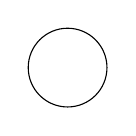
\begin{tikzpicture}
    \draw (0,0) circle (5mm);
  \end{tikzpicture}
  \caption{Un circulo en el margen}
\end{marginfigure}
\begin{nota}
En la versión para imprimir la tesis como un libro el margen se
reduce para permitir una caja de texto más grande, así las cosas que estén
en el margen podrían verse muy ``apretadas''.
\end{nota}

Por último en el código de este documento se puede ver que todas las
figuras tienen inmediatamente después del inicio del ambiente el comando
\verb|\centering|, debe ser este y no usar el ambiente \texttt{center}
para evitar espacios verticales no deseados. Además, como esto se hizo en
cada figura pudo haberse configurado en el preámbulo con el siguiente
comando
\begin{flushleft}
  \verb|\setfloatadjustment{figure}{\centering}|
\end{flushleft}
que también se puede usar en tablas, figuras al margen y los flotantes que
se hayan creado.


\section{Me falta desarrollar mejor}
Memoir puede crear glosarios de una forma muy similar a los índices. Se puede crear, por ejemplo, una lista de acrónimos y una de símbolos para
ejemplificar cómo se hacen. En el preámbulo se escribe
\begin{flushleft}
  \verb|\makeglossary[acro]|\\
  \verb|\makeglossary[simb]|
\end{flushleft}
Luego un acrónimo \verb|\glossary[acro]{HTML}{⟨HyperText Markup Language}| y un
símbolo \verb|\glossary[simb]{\(c\)}{Una constante importante}|. Por último,
en el lugar del documento donde vayan a ir los glosarios se escribe
\begin{flushleft}
  \verb|\clearpage %para crear una página nueva|\\
  \verb|\printglossary[acro]|\\
  \verb|\clearpage|\\
  \verb|\printglossary[simb]|
\end{flushleft}
Para cambiar el nombre del glosario, de la misma manera que en los índices, se usa
\begin{flushleft}
  \verb|\renewcommand{\glossaryname}{Un glosario}|
\end{flushleft}

La dificultad que encuentro en la creación de glosarios es la compilación.
Para esto también se usará \textit{makeindex}, pero si se intenta correr
este programa en alguno de los archivos para crear glosarios, por ejemplo
\begin{flushleft}
  \verb|makeindex acro.glo|
\end{flushleft}
se generaran muchos errores. Entonces, para lograr hacer estos glosarios se
necesita un archivo de configuración \texttt{basic.gst} que encontrarás en
los archivos de este proyecto y con esto la cadena de compilación que se usa para los glosarios es
\begin{flushleft}
  \verb|...|\\
  \verb|makeindex -s basic.gst -o acro.gls acro.glo|\\
  \verb|makeindex -s basic.gst -o simb.gls simb.glo|\\
  \verb|lualatex MiDocumento.tex|
\end{flushleft}
como no estoy seguro como llamar un archivo de configuración externo en
\texttt{arara} tuve que correr los dos \texttt{makeindex} en la terminal.

En overleaf (que usa \texttt{latemk}, pueden ver el archivo que usa para
compilar en \url{https://www.overleaf.com/learn/how-to/How_does_Overleaf_compile_my_project%3F}) tampoco funciona por defecto la
compilación de glosarios con el método de \textit{memoir}, aunque debería
ser posible configurarlo (me hace falta saber más de los archivos
\texttt{latexmkrc}). Por lo tanto sugeriré el paquete \texttt{glossaries} o
su versión extendida \texttt{glossaries-extra}. La versión extendida tiene
muchas capacidades con el método \texttt{bib2gls} pero tampoco es soportado
por overleaf, en este caso no será soportado por ningún método ya que usa
java y overleaf no soporta java (¿una implementación antigua de \LaTeX?).
Por lo que para hacer glosarios en overleaf hay que usar la versión simple
de \texttt{glossaries} que debería ser suficiente para una tesis.
